\section{Application 1} \label{sec:case_study1}

This section describes the results of the developed experiments in forecasting out-of-sample (test set). First, Section \ref{sec:E1} compares the results of evaluated models over ten datasets and three forecasting horizons adopted. In Tables \ref{tab:performancemeasure} and \ref{tab:performancemeasure2} in Appendix \ref{cs1_appendixB}, the best results regarding accuracy are presented in bold. Additionally, Figures~\ref{fig:PObrazil} and~\ref{fig:POusa} illustrate the relation between observed and predicted values achieved by models with the best set of performance measures depicted in Tables \ref{tab:performancemeasure} and \ref{tab:performancemeasure2}, as well as box-plots for out-of-sample errors, are illustrated in Figure \ref{fig:error}. Also, Figure~\ref{fig:importance} illustrates the variable importance of each input (both lags and exogenous inputs) used in the model's predictions.

\subsection{Performance measures for compared models \label{sec:E1}}

In this section, the main results achieved by the best model regarding \ac{sMAPE} and \ac{RRMSE} criteria are presented for short-term forecasting multi-days-ahead of cumulative cases of \ac{COVID-19} from five Brazilian and five American states. 

Firstly, considering the results for the Brazilian context, the main results are highlighted as follows.

\begin{itemize}
    \item \ac{AM}: In this state, \ac{VMD}--\ac{BRNN} could be considered to forecast \ac{COVID-19} cases, once the model outperformed all the single and \ac{VMD} models in both performance criteria in all forecasting horizons. The improvement in the \ac{sMAPE} achieved by \ac{VMD}--\ac{BRNN} ranges between 39.47\% - 96-06\%, 55.97\% - 94.88\%, and 67.41\% - 94.25\%, for \ac{ODA}, \ac{TDA}, and \ac{SDA} horizon respectively. Regarding \ac{RRMSE} analysis, the improvement ranges between 9.86\% - 94.81\%, 33.44\% - 93.29\%, and 56.66\% - 93.89\%, respectively.
    
    \item \ac{CE}, \ac{RJ}, and \ac{SP}: For these states, in all forecasting horizons, the \ac{VMD}--\ac{CUBIST} approach achieved better accuracy than other models, for both \ac{sMAPE} and \ac{RRMSE} criteria in the multi-days-ahead forecasting task of the confirmed number of \ac{COVID-19}. The improvement in \ac{sMAPE} ranges in 8.67\% - 96.57\%, 12.15\% - 97.78\%, and 59.37\% - 97.09\%, respectively, in \ac{ODA}, \ac{TDA}, and \ac{SDA} forecasting horizons. Moreover, the improvement in \ac{RRMSE} is ranged in 12.41\% - 97.32\%, 2.61\% - 98.29\%, and 49.99\% - 97.95\%, respectively.

    \item \ac{PE}: In this state, \ac{CUBIST} and \ac{SVR} present better performance to forecast \ac{COVID-19} cases. For \ac{ODA} and \ac{TDA}, \ac{CUBIST} outperforms models, while for \ac{SDA}, the \ac{SVR} achieves better accuracy regarding \ac{sMAPE} and \ac{RRMSE} than others. The improvement in the \ac{sMAPE} for \ac{ODA} and \ac{TDA} achieved by \ac{CUBIST} ranges between 6.81\% - 97.93\%, and 24.94\% - 98.23\%, respectively. For \ac{SDA}, \ac{SVR} outperforms other models, and this criterion is reduced in the range of 49.36\% - 98.27\%. Moreover, the same behavior is observed when the improvement in the \ac{RRMSE} criterion is obtained.
\end{itemize}

\textbf{Remark:} In this experiment, regarding the Brazilian states, 150 scenarios (5 datasets, 3 forecasting horizons, and 10 models) were evaluated for the task of forecasting cumulative \ac{COVID-19} cases. In an overview, the best models for each state, obtained \ac{sMAPE} ranged between 1.14\% - 3.05\%, 1.06\% - 2.79\%, and 1.05\% - 3.03\% for \ac{ODA}, \ac{TDA}, and \ac{SDA} forecasting, respectively. In the Brazilian context, the ranking of the model in all scenarios is \ac{VMD}--\ac{CUBIST}, \ac{VMD}--\ac{BRNN}, \ac{SVR}, \ac{CUBIST}, \ac{VMD}--\ac{SVR}, \ac{BRNN}, \ac{VMD}--\ac{QRF}, \ac{QRF}, \ac{VMD}--\ac{KNN}, and \ac{KNN}. From a broader perspective, the efficiency of the \ac{VMD} models is due to the approach's capability to deal with the non-linearity and non-stationarity of the data. Moreover, the efficiency of the \ac{CUBIST} is due mainly to its ensemble learning of rules, in which the approach takes advantage of each rule based on the input set. On the other hand, the difficulty of the \ac{KNN} model to forecast cumulative \ac{COVID-19} cases could be attributed to the fact that this approach requires more observations to effectively learn the data pattern once an average of past similar values obtains the forecasting. 

In the next, considering the results for the \ac{USA} context, the main results are highlighted as follows.

\begin{itemize}
    \item \ac{CA}: In \ac{CA} state, \ac{BRNN} outperformed other models, in all forecasting horizons, for both \ac{sMAPE} and \ac{RRMSE} criteria. In this aspect, the improvement in \ac{sMAPE} ranges between 29.98\% - 97.86\%, 4.64\% - 97.71\%, and 48.56\% - 97.99\%, for \ac{ODA}, \ac{TDA}, and \ac{SDA}, respectively. Regarding \ac{RRMSE}, the improvement ranges in 24.00\% - 97.67\%, 6.57\% - 97.78\%, and 48.62\% - 98.11\%, respectively.
    
    \item \ac{IL}, \ac{MA}, and \ac{NJ}: For both performance criteria, \ac{CUBIST} outperformed other models in \ac{ODA}, for \ac{IL} and \ac{NJ} states, and \ac{TDA}, for \ac{IL}. \ac{BRNN} presented better accuracy than other models, for \ac{MA} state in \ac{ODA} and \ac{TDA}. Moreover, \ac{VMD}--\ac{CUBIST} outperformed other models in \ac{SDA} for these three states. The improvement in \ac{sMAPE} ranges in 6.63\% - 98.76\%, 31.89\% - 98.09\%, and 3.76\% - 97.98\%, respectively, in \ac{ODA}, \ac{TDA}, and \ac{SDA} forecasting horizons. Moreover, regarding the \ac{RRMSE}, the improvement ranges between 7.54\% - 98.48\%, 0.83\% - 98.25\%, and 3.25\% - 98.11\%, respectively.
    
    \item \ac{NY}: For \ac{NY} state, in both performance criteria, \ac{VMD}--\ac{CUBIST} presented better accuracy than other models in \ac{ODA} forecasting. In contrast, \ac{SVR} outperformed the other models in \ac{TDA} and \ac{SDA} forecasting. Regarding \ac{sMAPE}, the improvement ranges 17.86\% - 95.44\%, 16.12\% - 95.69\%, and 42.39\% - 92.71\%, for \ac{ODA}, \ac{SDA}, and \ac{TDA}, respectively. For \ac{RRMSE}, the improvement ranges 25.78\% - 96.09\%, 7.78\% - 95.43\%, and 43.76\% - 93.45\%, respectively.
\end{itemize}

\textbf{Remark:} In this experiment, regarding the American states, 150 scenarios (5 datasets, 3 forecasting horizons, and 10 models) were evaluated for the task of forecasting cumulative \ac{COVID-19} cases. In an overview, the best models for each state, obtained \ac{sMAPE} ranged between 0.54\% - 1.90\%, 0.55\% - 1.59\%, and 0.62\% - 3.08\% for \ac{ODA}, \ac{TDA}, and \ac{SDA} forecasting, respectively. In the American context, the ranking of the models in all scenarios is \ac{VMD}--\ac{CUBIST}, \ac{BRNN}, \ac{CUBIST}, \ac{SVR}, \ac{VMD}--\ac{BRNN}, \ac{VMD}--\ac{SVR}, \ac{VMD}--\ac{QRF}, \ac{QRF}, \ac{KNN}, and \ac{VMD}--\ac{KNN}. The same behavior in Brazilian cases is shown in the American, in which the \ac{VMD}--\ac{CUBIST} overall had better average performance than the other models.

\subsection{Graphical analysis}

According to the information depicted in Figures \ref{fig:PObrazil} and \ref{fig:POusa}, it is possible to identify that the behavior of the data is learned by the evaluated models, which can forecast compatible cases with the observed values. In most states, the satisfactory performance presented in the training stage persists in the test phase. In Figures \ref{subfig:AM}, \ref{subfig:PE}, \ref{subfig:CA}, and \ref{subfig:NY}, the models presented some difficulties in capturing the behavior of the data in the training stage, however, in the test phase, the models could perform accurately showing low errors. 

% BRA states
\begin{figure}[htb!]
    \centering
    \subfloat[AM \label{subfig:AM}]{
    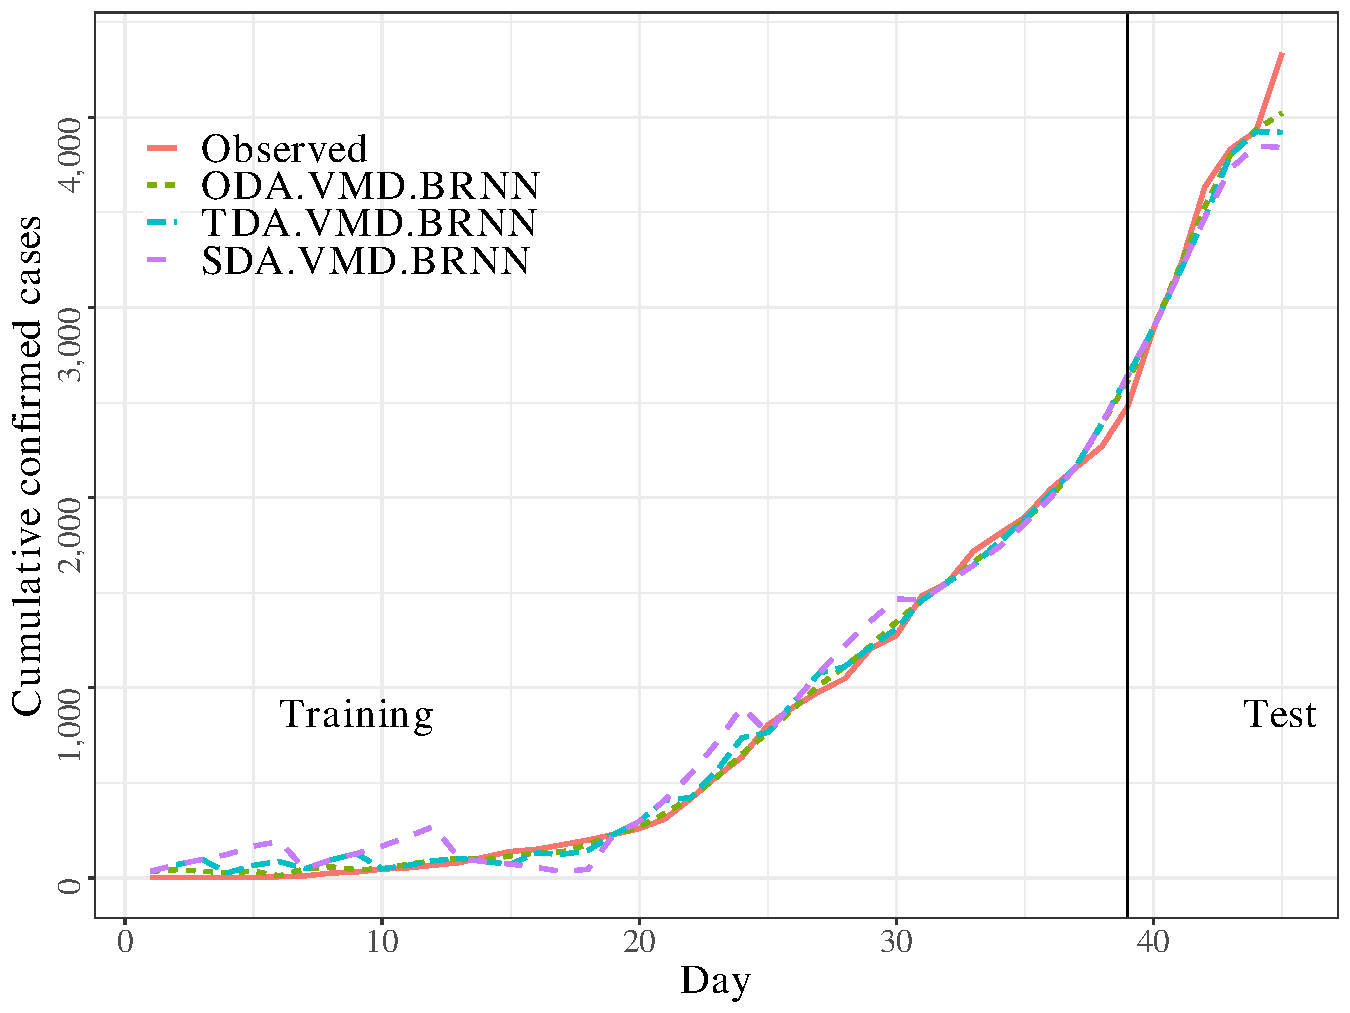
\includegraphics[width=0.43\linewidth]{Media/cs1_PO_AM.pdf}
    }
    %
    \subfloat[CE \label{subfig:CE}]{
    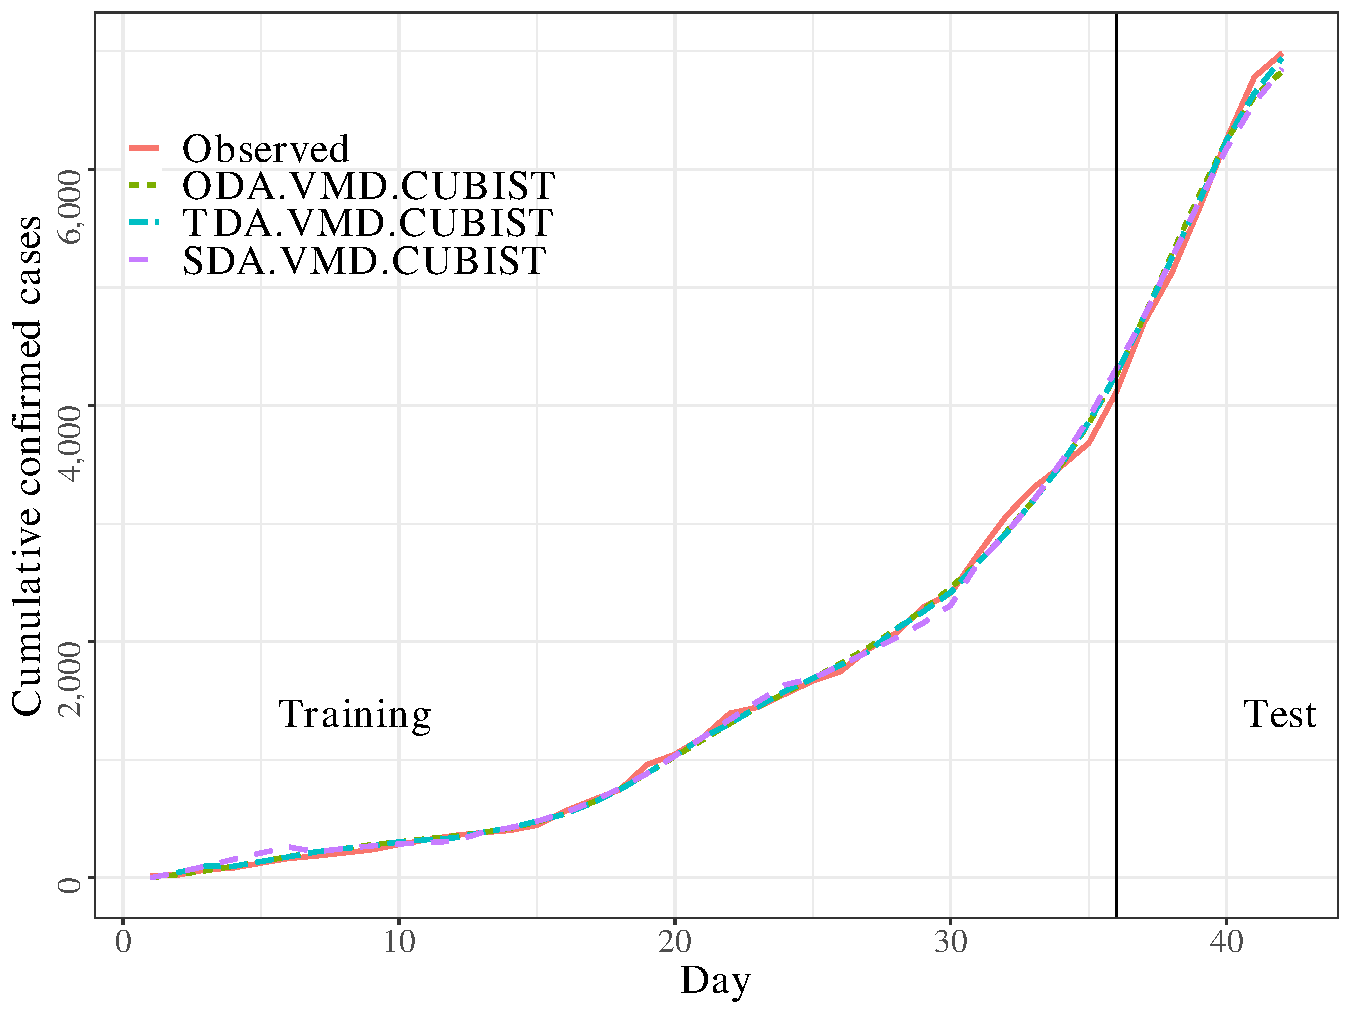
\includegraphics[width=0.43\linewidth]{Media/cs1_PO_CE.pdf}
    }
    
    \subfloat[PE \label{subfig:PE}]{
    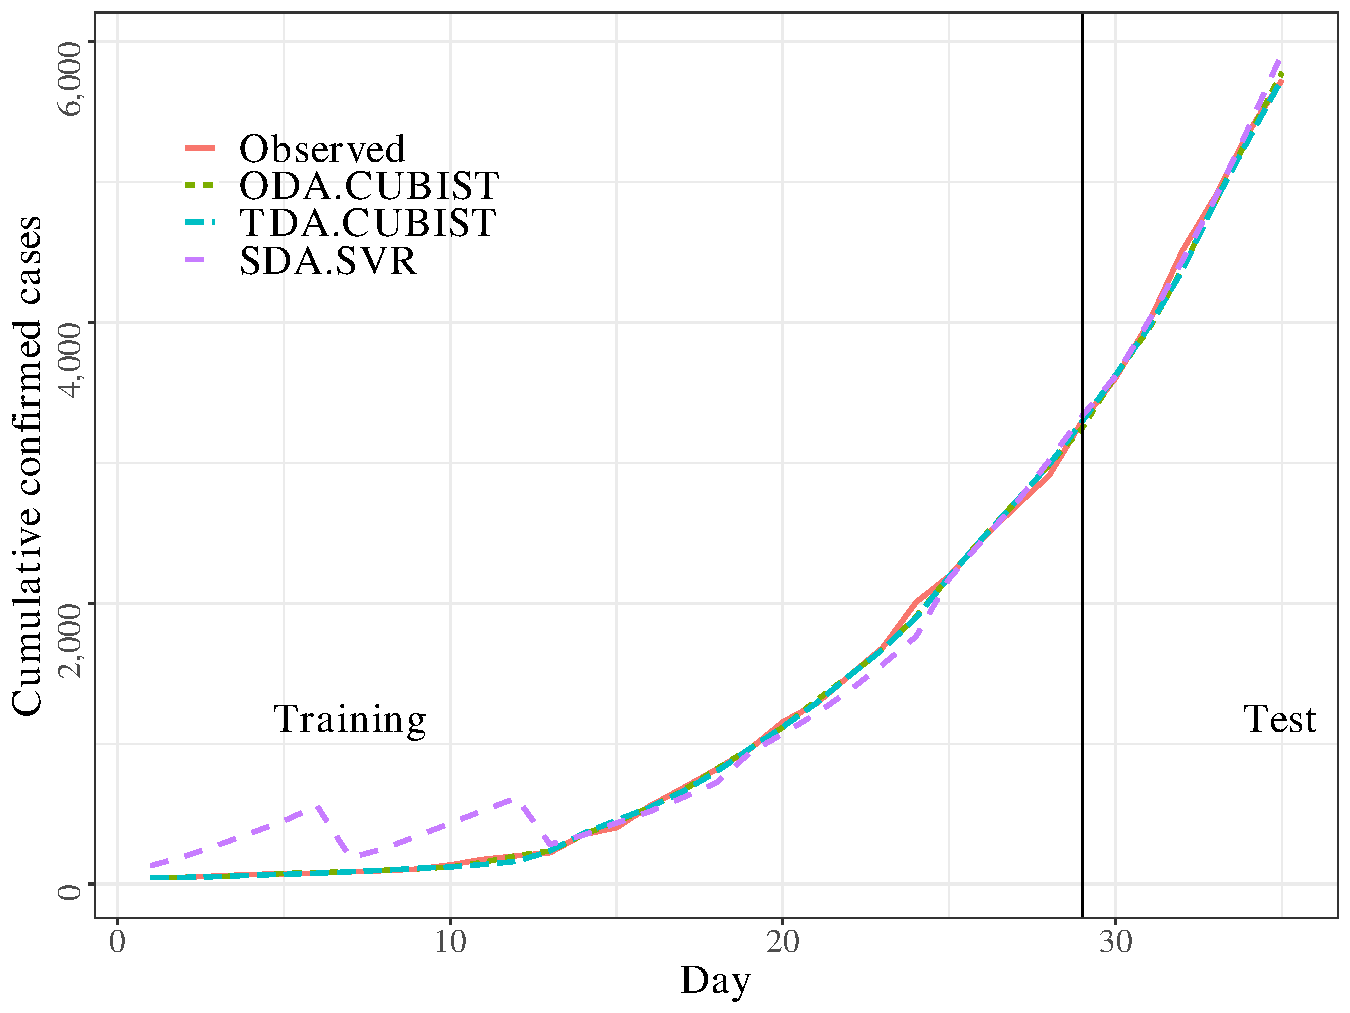
\includegraphics[width=0.43\linewidth]{Media/cs1_PO_PE.pdf}
    }
    %
    \subfloat[RJ \label{subfig:RJ}]{
    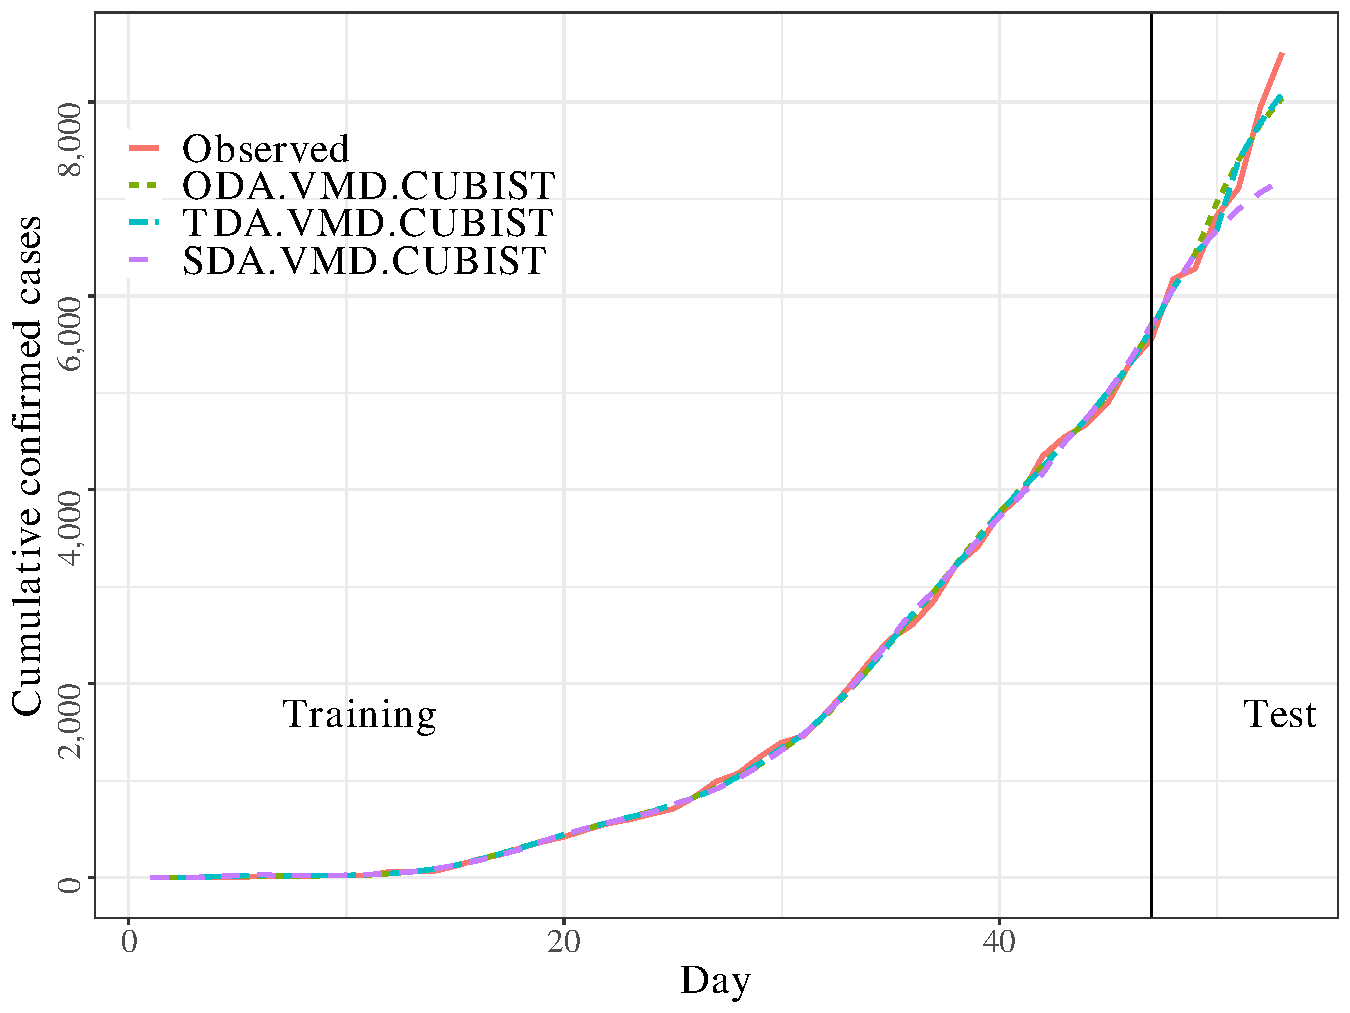
\includegraphics[width=0.43\linewidth]{Media/cs1_PO_RJ.pdf}
    }
    
    \subfloat[SP \label{subfig:SP}]{
    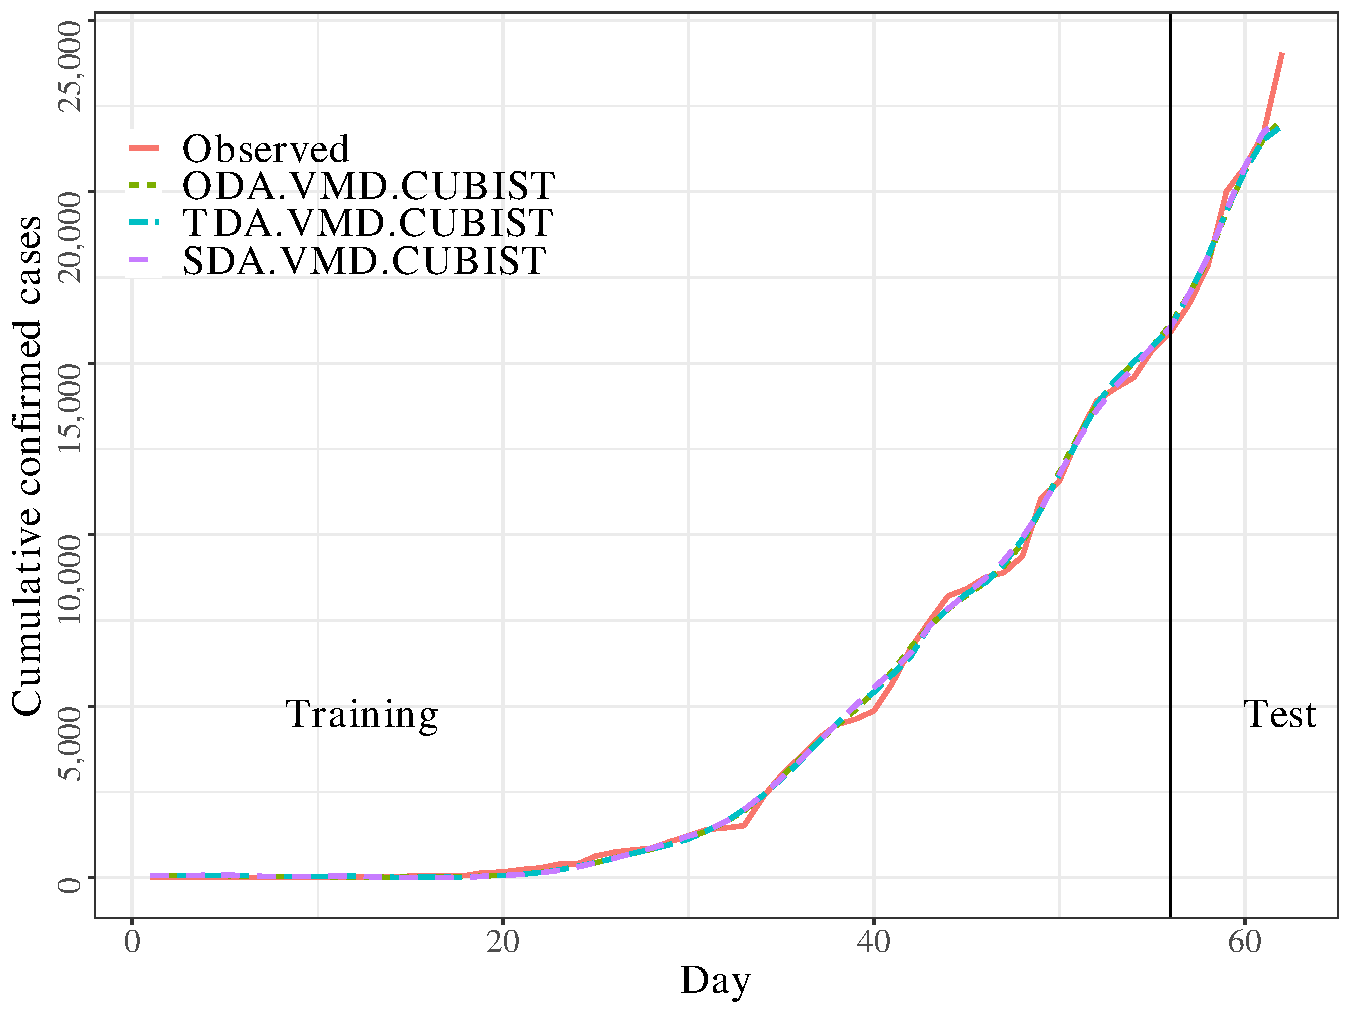
\includegraphics[width=0.43\linewidth]{Media/cs1_PO_SP.pdf}
    }
    %
    \caption{Prediction versus observed COVID-19 cases for Brazilian States}
    \label{fig:PObrazil}
    \source{\citeonline{dasilva2022Multistep}}
\end{figure}

% USA states
\begin{figure}[htb!]
    \centering
    \subfloat[CA \label{subfig:CA}]{
    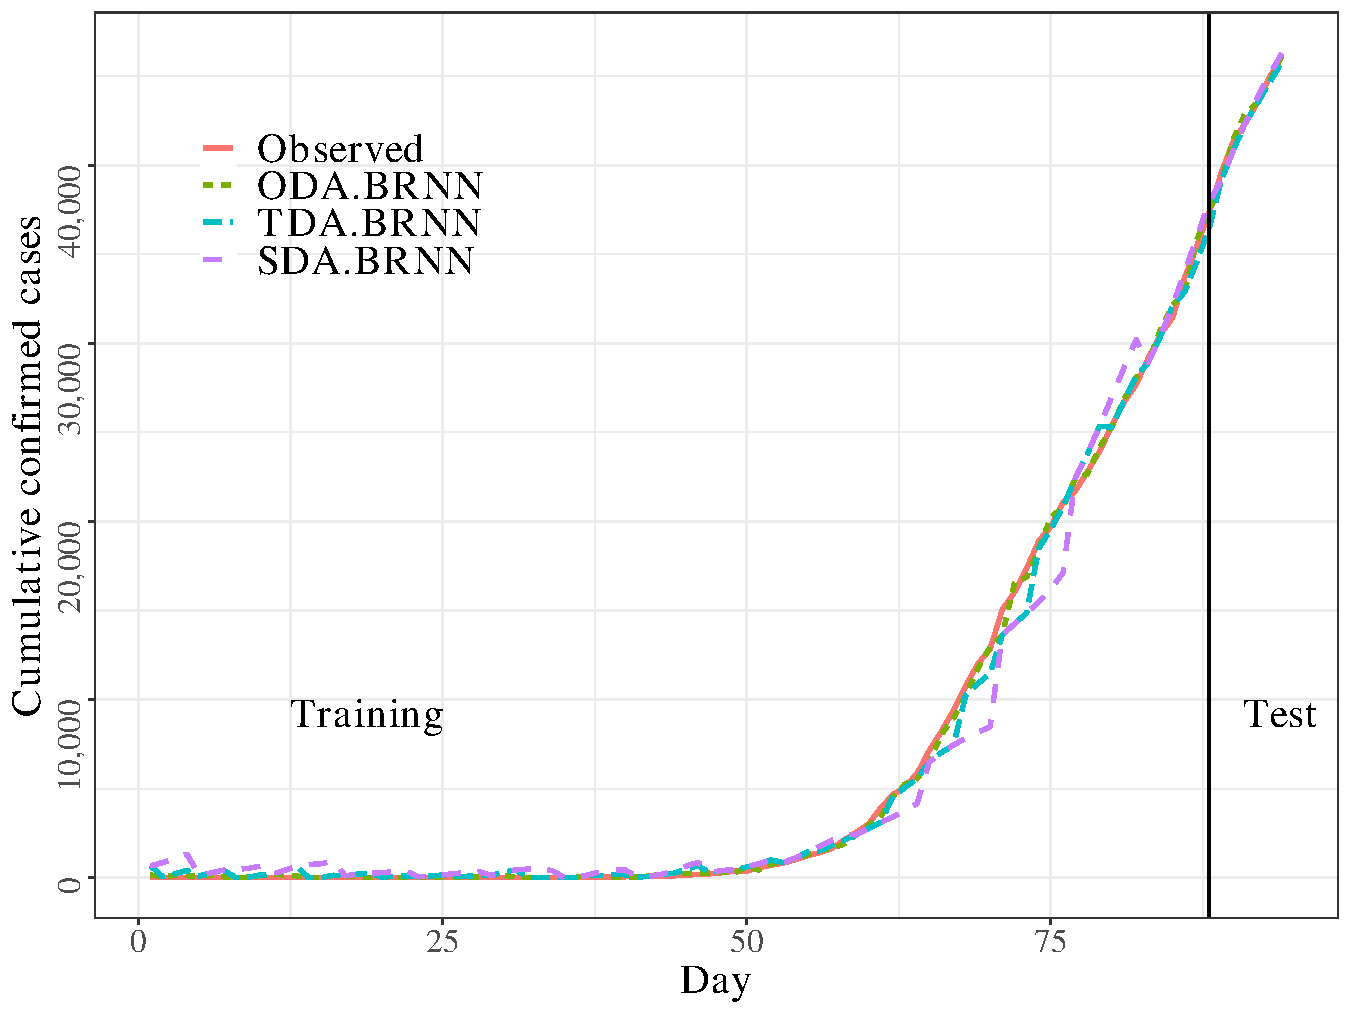
\includegraphics[width=0.43\linewidth]{Media/cs1_PO_CA.pdf}
    }
    %
    \subfloat[IL \label{subfig:IL}]{
    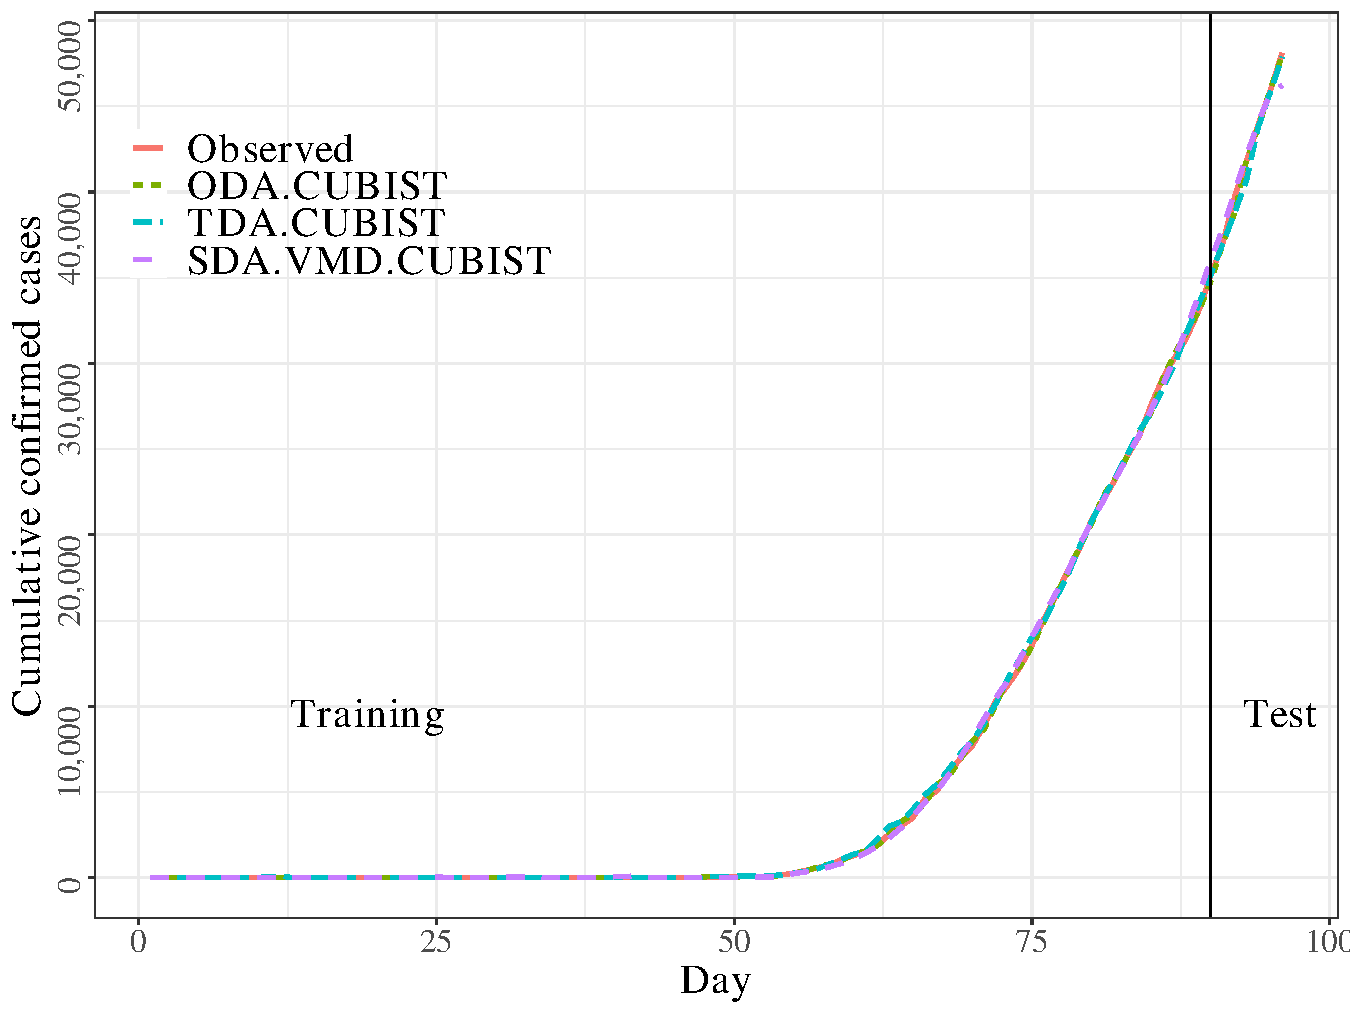
\includegraphics[width=0.43\linewidth]{Media/cs1_PO_IL.pdf}
    }

    \subfloat[MA \label{subfig:MA}]{
    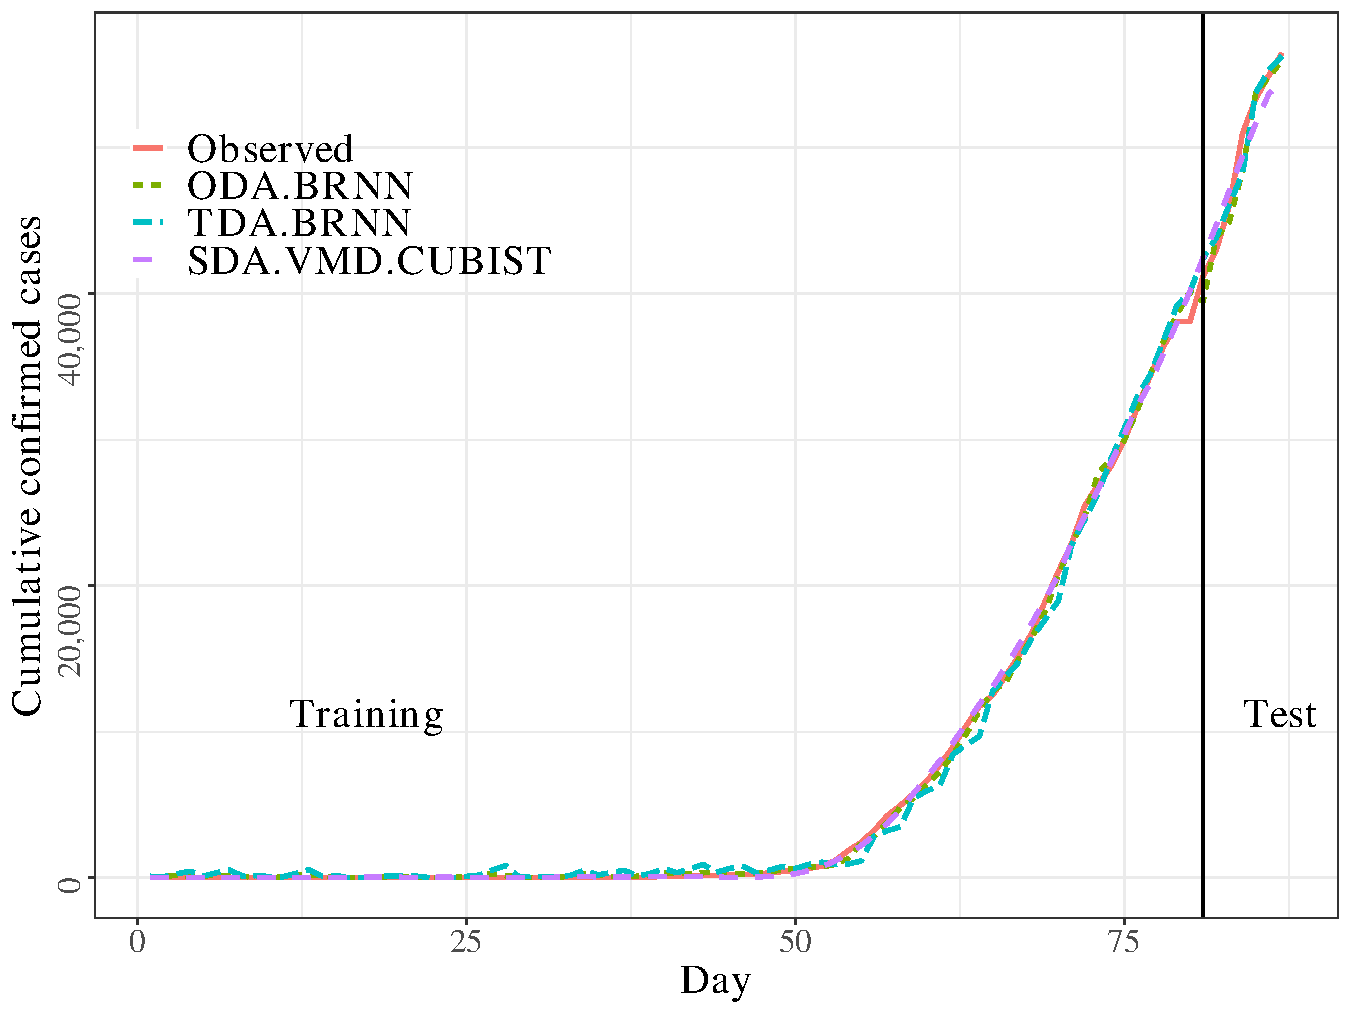
\includegraphics[width=0.43\linewidth]{Media/cs1_PO_MA.pdf}
    }
    %
    \subfloat[NJ \label{subfig:NJ}]{
    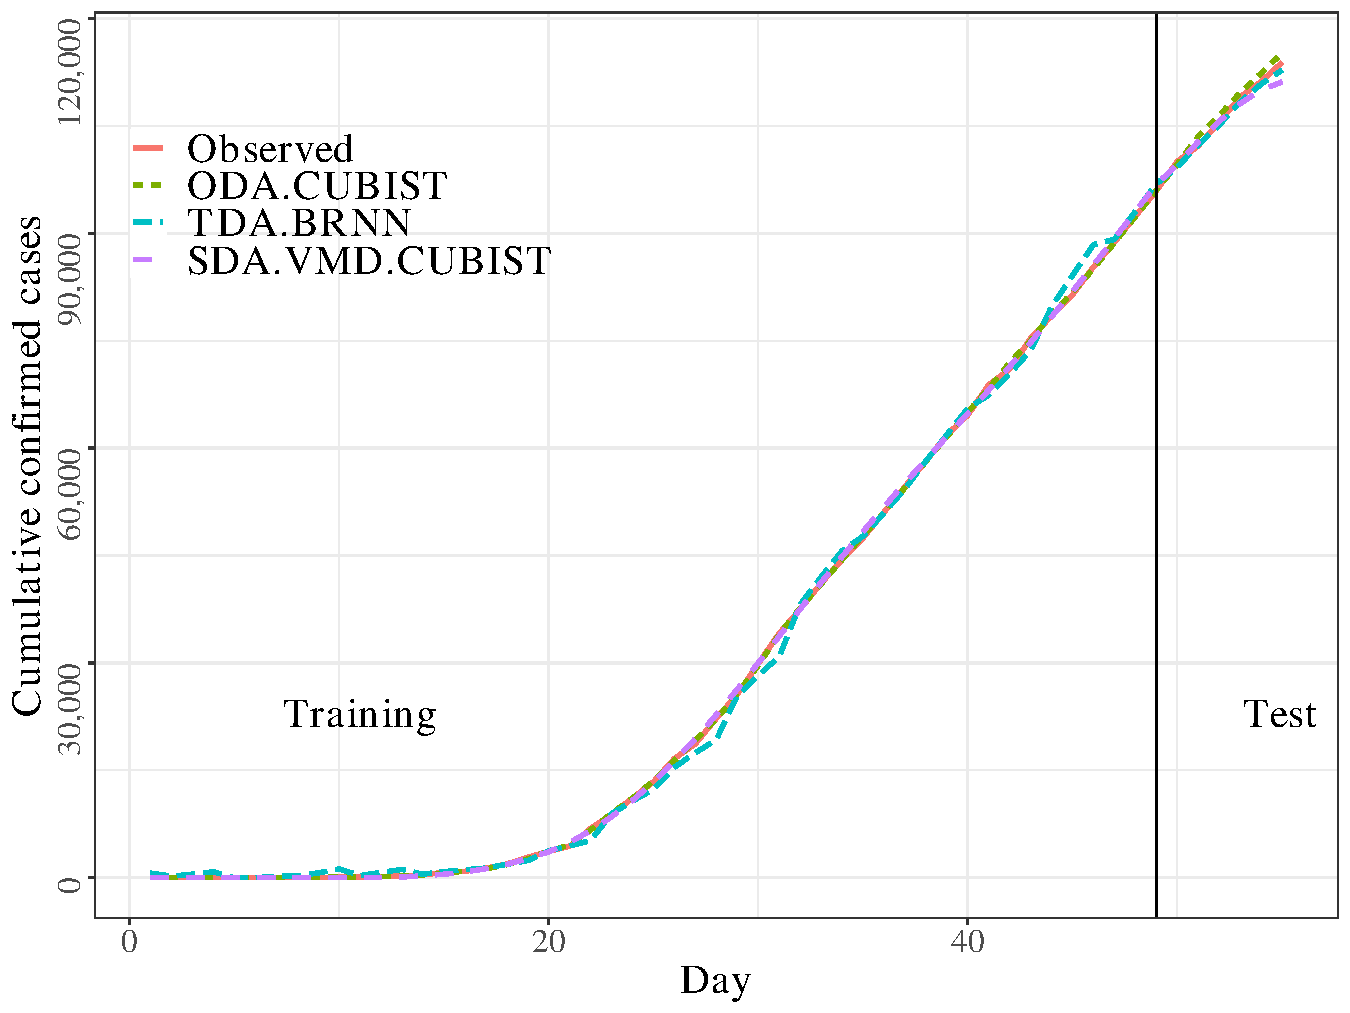
\includegraphics[width=0.43\linewidth]{Media/cs1_PO_NJ.pdf}
    }
    
    \subfloat[NY \label{subfig:NY}]{
    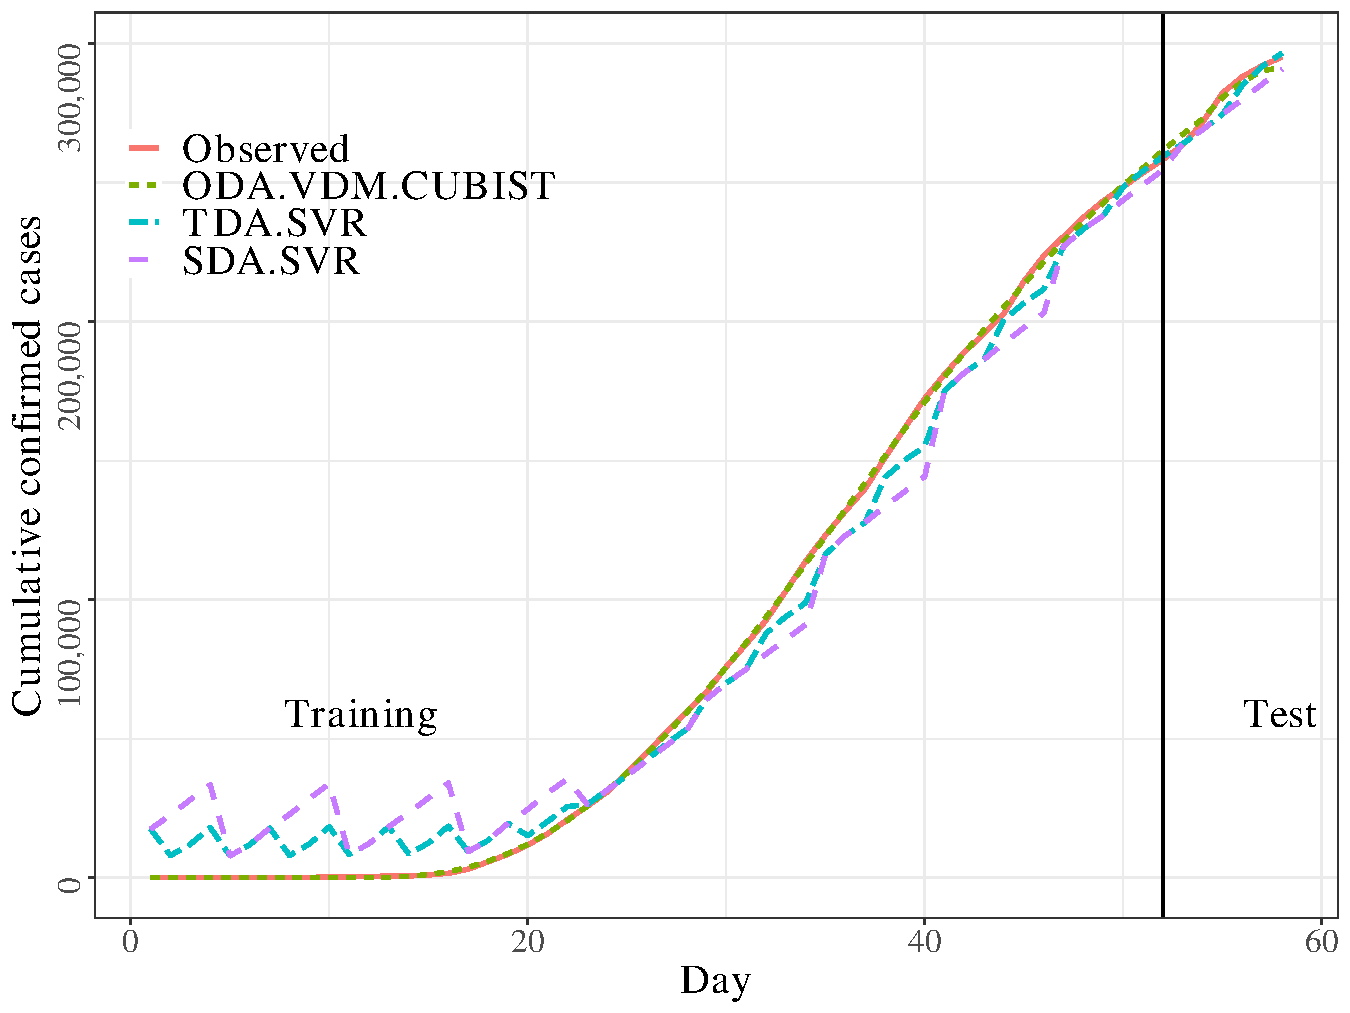
\includegraphics[width=0.43\linewidth]{Media/cs1_PO_NY.pdf}
    }
    \caption{Prediction versus observed COVID-19 cases for American States}
    \label{fig:POusa}
    \source{\citeonline{dasilva2022Multistep}}
\end{figure}

Furthermore, Figure \ref{fig:error} presents the box-plots of test set forecasting errors in the \ac{SDA} horizon for each model and each state. Due to the recursive strategy adopted, the \ac{SDA} horizon was chosen for the analysis once the errors tend to grow as the forecast horizon increases. The box diagram depicts the variation of absolute errors for each model, which reflects the stability of each model. In this context, the dots out of boxes are considered outliers errors.

% Box plot
\begin{figure}[htb!]
    \centering
    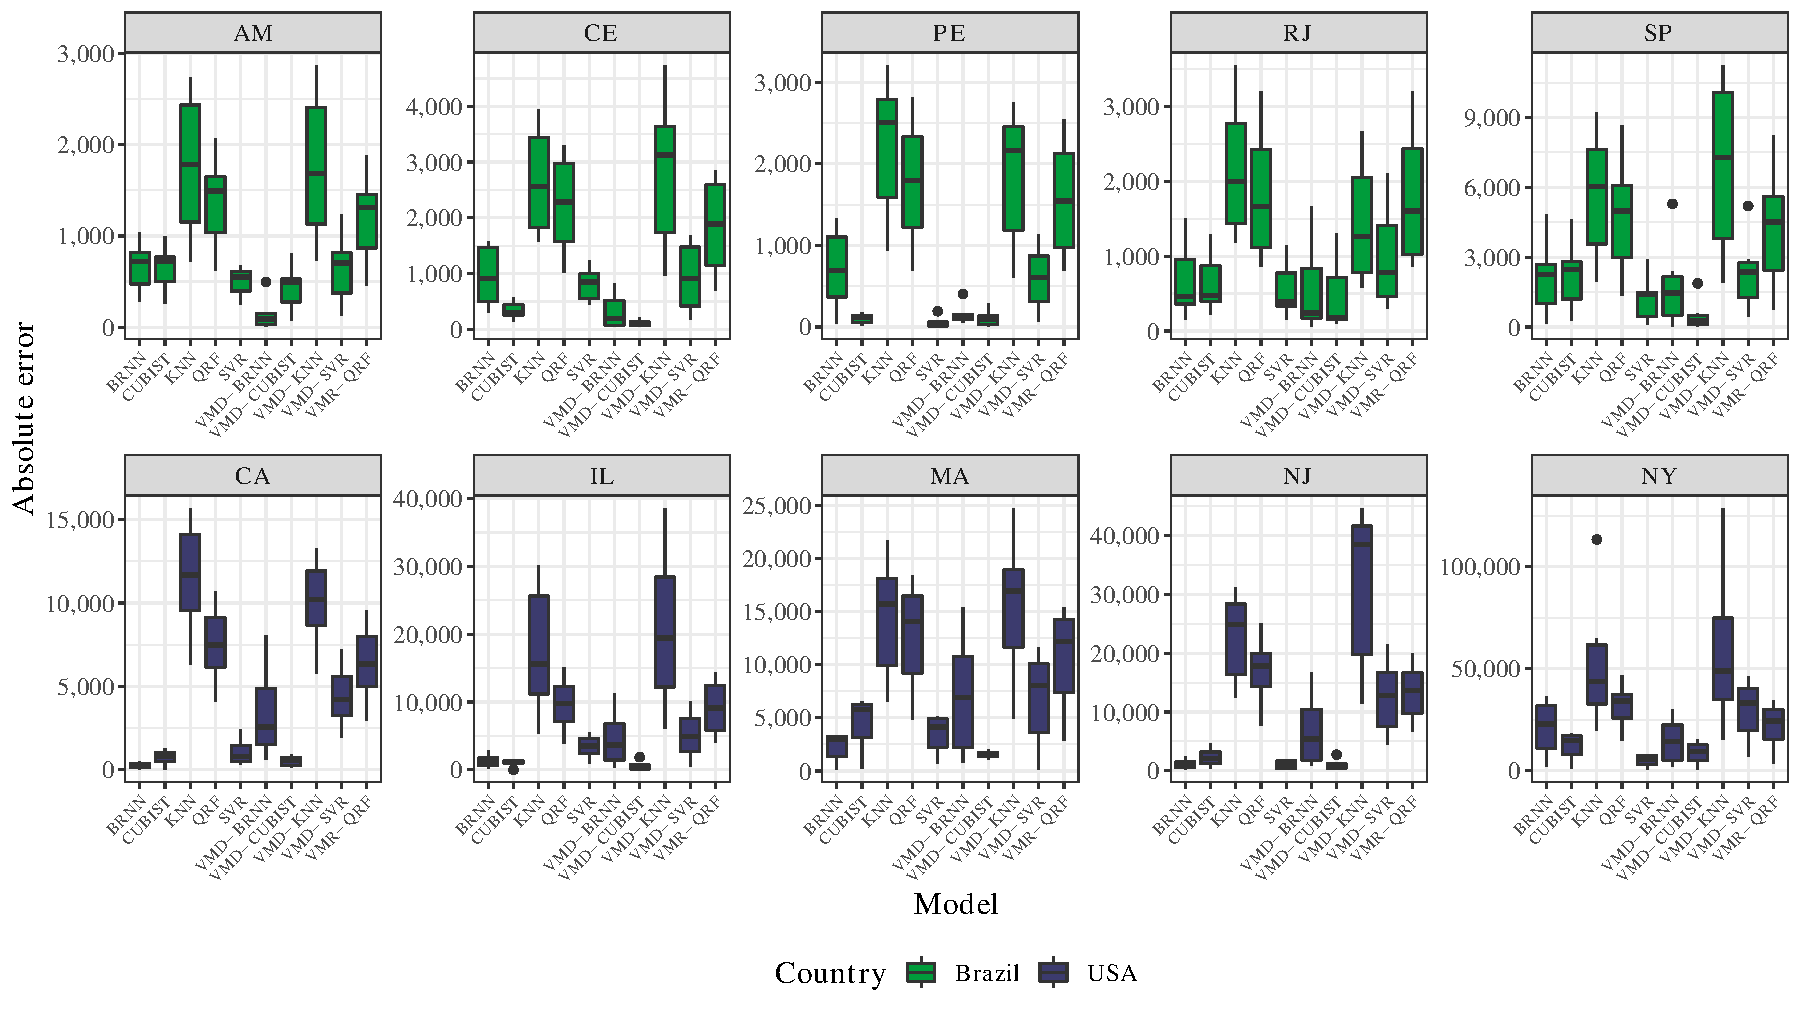
\includegraphics[width=\linewidth]{Media/cs1_error.pdf}
    \caption{Box-plot for absolute error according to model and state for COVID-19 forecasting for SDA}
    \label{fig:error}
    \source{\citeonline{dasilva2022Multistep}}
\end{figure}

Through the box-plot analysis, models with lower variation in the errors are indicated by the boxes with a smaller size. Figure \ref{fig:error} corroborates the results presented in Tables \ref{tab:performancemeasure} and \ref{tab:performancemeasure2}. Models with lower errors achieve better stability, which means that the most appropriate model for each state can maintain a learning pattern, obtaining homogeneous forecasting errors.

The variable importance quantifies the relationship between the predictor variables (inputs) and the predicted value. Finally, Figure \ref{fig:importance} is presented the variable importance of each input used to fit and train the models. As expected, the lag inputs show high significance due to their high correlation to the output. However, it is essential to notice that climate data presented some influence in predicting \ac{COVID-19} cumulative cases, especially in the Brazilian context, that the variance of the Temperature data reaches up to 50\% of importance. In other words, the exogenous climatic inputs are at some level relevant to predicting cumulative cases of \ac{COVID-19} in Brazil's and \ac{USA}'s context for the five evaluated states.

% Importance
\begin{figure}[htb!]
    \centering
    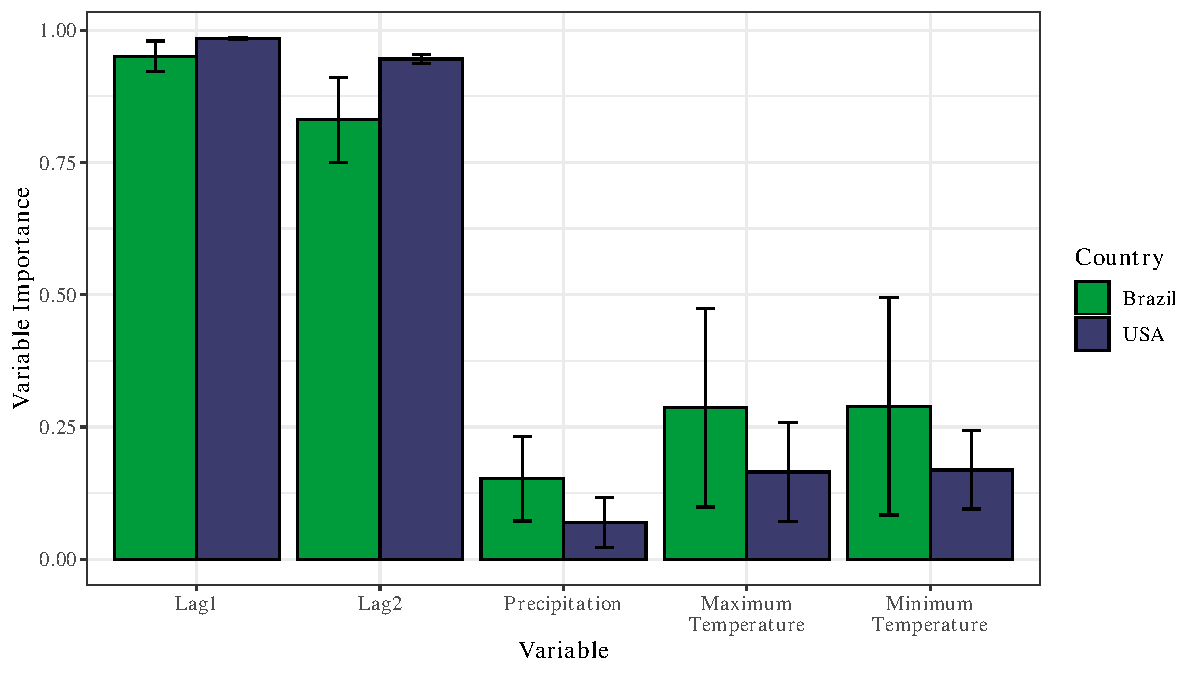
\includegraphics[width=0.8\linewidth]{Media/cs1_importance.pdf}
    \caption{Variable importance for Brazil and USA}
    \label{fig:importance}
    \source{\citeonline{dasilva2022Multistep}}
\end{figure}

\subsection{Conclusions of the Application 1 \label{CONC}}

In this study, machine learning approaches named \ac{BRNN}, \ac{CUBIST}, \ac{KNN}, \ac{QRF}, and \ac{SVR}, as well as \ac{VMD} approach, were employed in the task of forecasting one, three, and six-days-ahead the \ac{COVID-19} cumulative confirmed cases in five Brazilian states and five American states with a high daily incidence. The \ac{COVID-19} cumulative confirmed cases for \ac{AM}, \ac{CE}, \ac{PE}, \ac{RJ}, and \ac{SP} states, and \ac{CA}, \ac{IL}, \ac{MA}, \ac{NJ}, and \ac{NY} were used. The \ac{IP}, \ac{sMAPE}, and \ac{RRMSE} criteria were adopted to evaluate the performance of the compared approaches. The stability of out-of-sample errors was evaluated through box-plots. Further, the variable importance of the lag and exogenous climatic inputs were analyzed.

Considering the \textbf{RQ 1.1} - \textit{Can signal decomposition approaches enhance the performance of forecasting \ac{COVID-19} cumulative cases time series?}, it is possible to infer that \ac{CUBIST} coupled with the \ac{VMD} model are suitable tools to forecast \ac{COVID-19} cases for most of the adopted states once these approaches were able to learn the non-linearities inherent to the evaluated epidemiological time series. Also, \ac{BRNN} and \ac{SVR} models deserve attention for developing this task. Therefore, the ranking of models in all scenarios for Brazilian states is \ac{VMD}--\ac{CUBIST}, \ac{VMD}--\ac{BRNN}, \ac{SVR}, \ac{CUBIST}, \ac{VMD}--\ac{SVR}, \ac{BRNN}, \ac{VMD}--\ac{QRF}, \ac{QRF}, \ac{VMD}--\ac{KNN}, and \ac{KNN}, and for \ac{USA} states is \ac{VMD}--\ac{CUBIST}, \ac{BRNN}, \ac{CUBIST}, \ac{SVR}, \ac{VMD}--\ac{BRNN}, \ac{VMD}--\ac{SVR}, \ac{VMD}--\ac{QRF}, \ac{QRF}, \ac{KNN}, and \ac{VMD}--\ac{KNN}. Also, looking for \ac{COVID-19} forecasts six days ahead, hybrid models are more suitable tools than non-decomposed models. Further to answer \textbf{RQ 2} - \textit{How does the use of exogenous features impact performance improvement when forecasting \ac{COVID-19} cumulative cases time series?}, it was observed that climatic variables, such as temperature and precipitation, indeed influence increasing the accuracy when predicting \ac{COVID-19} cases, wherein some cases climate inputs reached up to 50\% of importance in the forecasting model. To answer \textbf{RQ 1.1} and \textbf{RQ 2} the specific objectives \textbf{\ref{obj_a}} and \textbf{\ref{obj_c}} were achieved.